\chapter{Исследовательская часть}

В данном разделе будут приведены результаты работы разработанного программного обеспечения и поставлен эксперимент по оценке эффективности работы программы.

\section{Результаты работы программного обеспечения}

На рисунке \ref{img:t1} приведен результат генерации сцены, на которой показана молния-лидер.

\begin{figure}[H]
	\begin{center}
		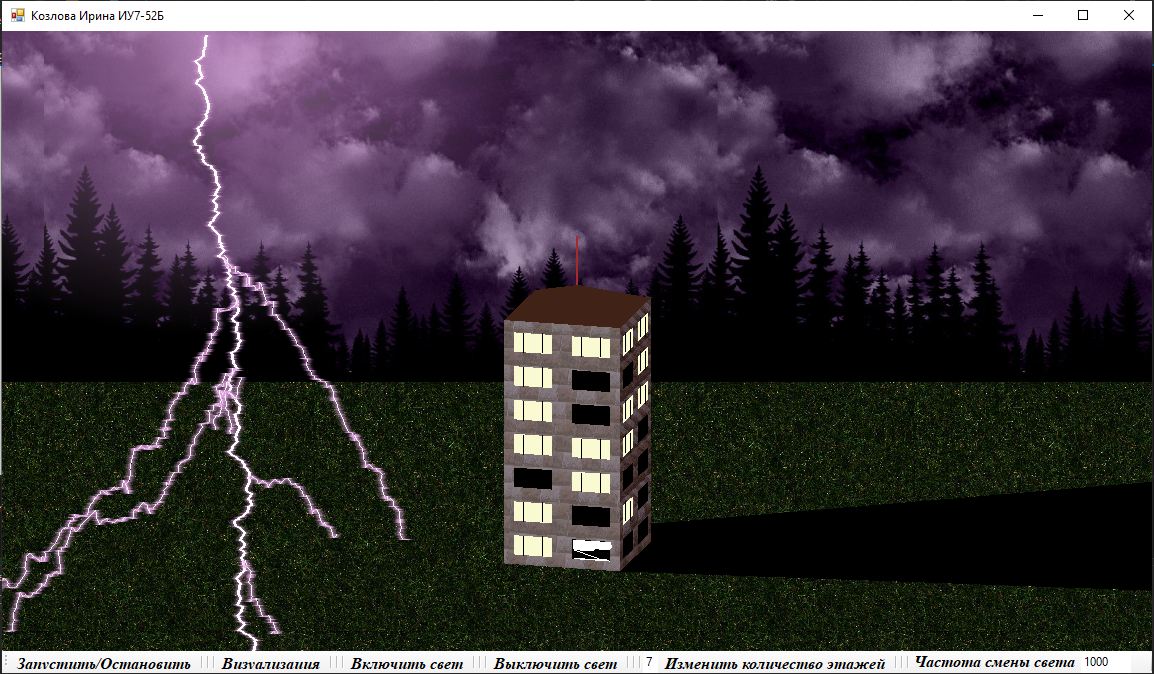
\includegraphics[scale=0.38]{img/prog_res/t1.png}
	\end{center}
	\captionsetup{justification=centering}
	\caption{Изображение с молнией-лидером}
	\label{img:t1}
\end{figure}

На изображении \ref{img:t2} приведен результат генерации сцены, на котором видно отражение молнии от стекл окон дома.

\begin{figure}[H]
	\begin{center}
		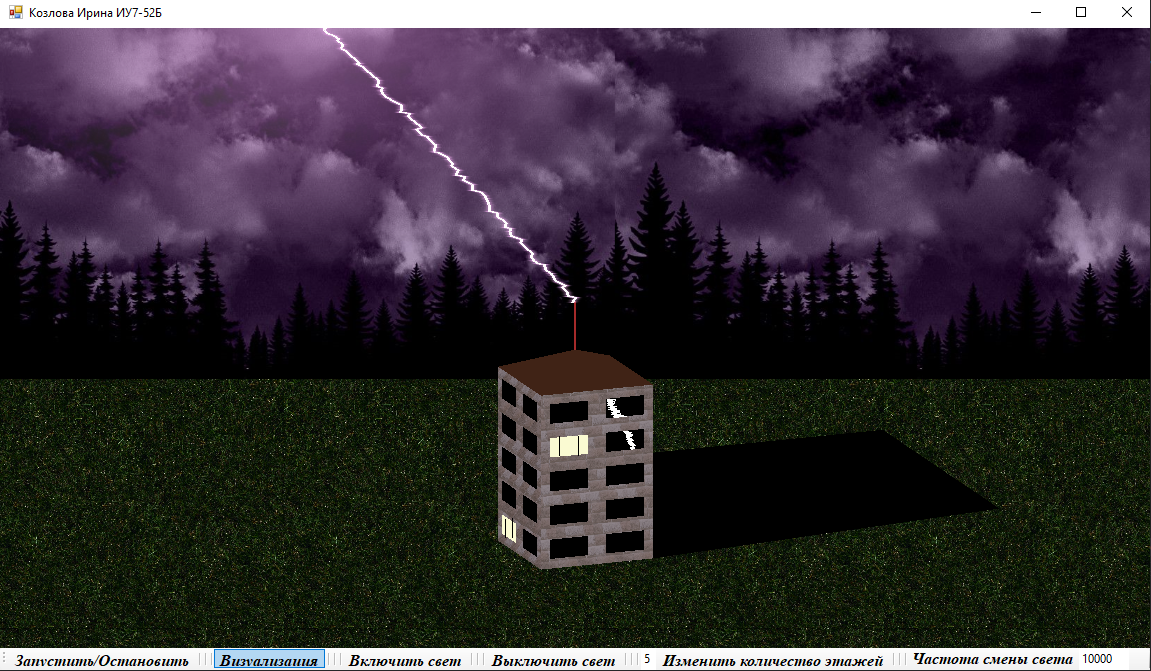
\includegraphics[scale=0.38]{img/prog_res/t2.png}
	\end{center}
	\captionsetup{justification=centering}
	\caption{Изображение с отражением молнии от стекл окон дома}
	\label{img:t2}
\end{figure}

На изображении \ref{img:t3} приведен результат генерации сцены, на которой показана молния, бьющая в громоотвод.

\begin{figure}[H]
	\begin{center}
		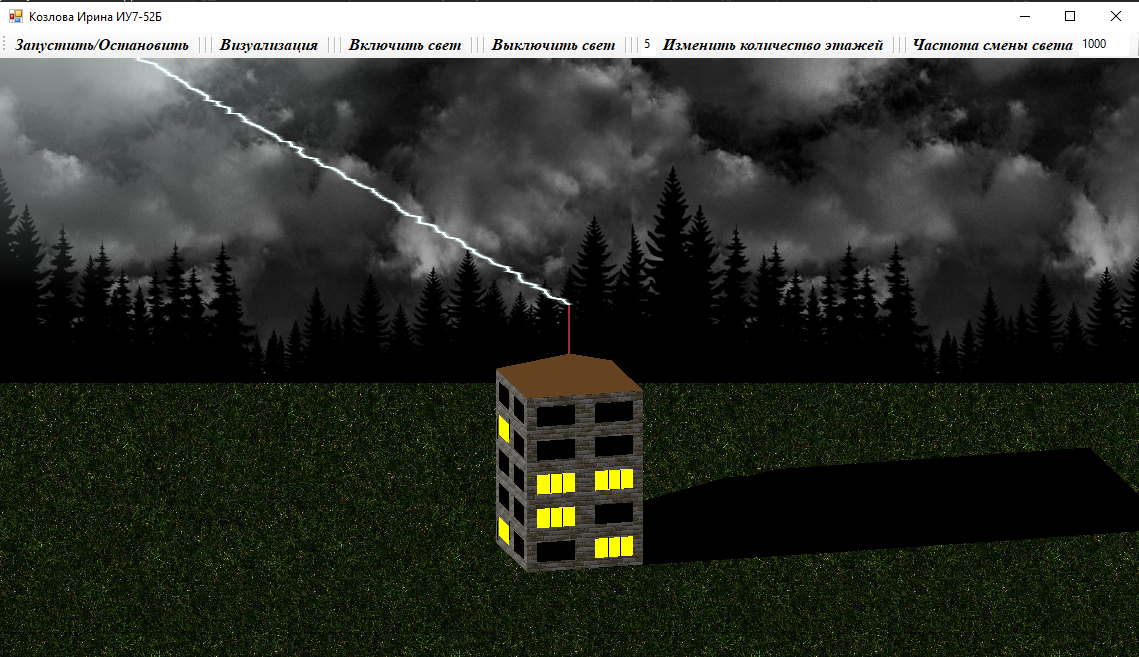
\includegraphics[scale=0.38]{img/prog_res/t3.png}
	\end{center}
	\captionsetup{justification=centering}
	\caption{Изображение с молнией, бьющей в громоотвод}
	\label{img:t3}
\end{figure}

На изображении \ref{img:t4} приведен результат генерации сцены, на которой показана молния с большим количеством побочных ветвей.

\begin{figure}[H]
	\begin{center}
		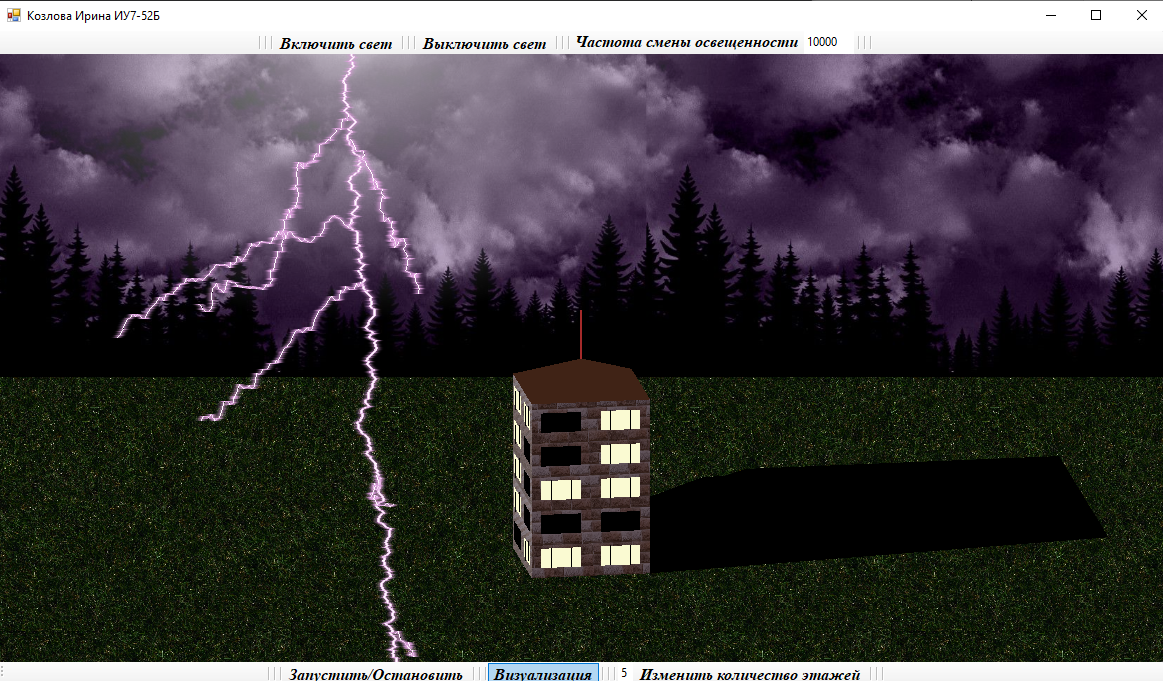
\includegraphics[scale=0.38]{img/prog_res/t4.png}
	\end{center}
	\captionsetup{justification=centering}
	\caption{Изображение с молнией, у которой большое количество ветвей}
	\label{img:t4}
\end{figure}

\section{Технические характеристики}

Технические характеристики устройства, на котором выполнялось тестирование, следующие.

\begin{itemize}
	\item Операционная система: Windows 10 \cite{oswind} x86\_64.
	\item Память: 8 GiB.
	\item Процессор: 11th Gen Intel® Core™ i5-1135G7 @ 2.40GHz \cite{intel}.
	\item 4 физических ядра и 8 логических ядра.
\end{itemize}

Тестирование проводилось на ноутбуке, включенном в сеть электропитания. Во время тестирования ноутбук был нагружен только встроенными приложениями окружения, а также непосредственно системой тестирования.


\section{Постановка эксперимента} 

\subsection{Цель эксперимента}
Целью эксперимента является попытка оптимизировать алгоритм обратной трассировки лучей для данной сцены. 

Необходимо провести теоретическое сравнение оптимизированного и неоптимизированного алгоритма, а также подтвердить результаты на практике путем подсчета количесва испускаемых лучей для построения сцены.

Эксперимент будет проводиться на различных сценах, с разным количесвом этажей, а также с разными видами молнии.
\begin{enumerate}
	\item Количество этажей -- 6, молния без побочных ветвей бьет в громоотвод, количество окон, в которых горит цвет -- не имеет значения.
	\item Количество этажей -- максимальное, молния-лидер с большим количеством ветвей бьет в землю, во всех окнах не горит свет.
	\item Количество этажей -- минимальное, молния без ветвей бьет в громоотвод, во всех окнах горит свет. 
	\item Количество этажей -- 5, молния-лидер бьет в землю, количество окон, в которых горит свет -- не имеет значение.
	\item Количество этажей -- максимальное, молния-лидер бьет в землю, во всех окнах горит свет.
\end{enumerate}

Также будет приведены:
\begin{itemize}
	\item график зависимости количества испускаемых лучей от количества окон, в которых не горит свет (учитываются только те окна, которые  ''видны'' пользователю);
	\item график зависимости времени построения от количества окон, в которых не горит свет.
\end{itemize}


\subsection{Теоретическое сравнение алгоритма трассировки лучей}

\subsubsection{Сцена 1}

\textbf{Описание}: Количество этажей -- 6, молния без побочных ветвей бьет в громоотвод, количество окон, в которых горит цвет -- не имеет значения.

Результат представлен на рисунке \ref{img:s1}.
\begin{figure}[H]
	\begin{center}
		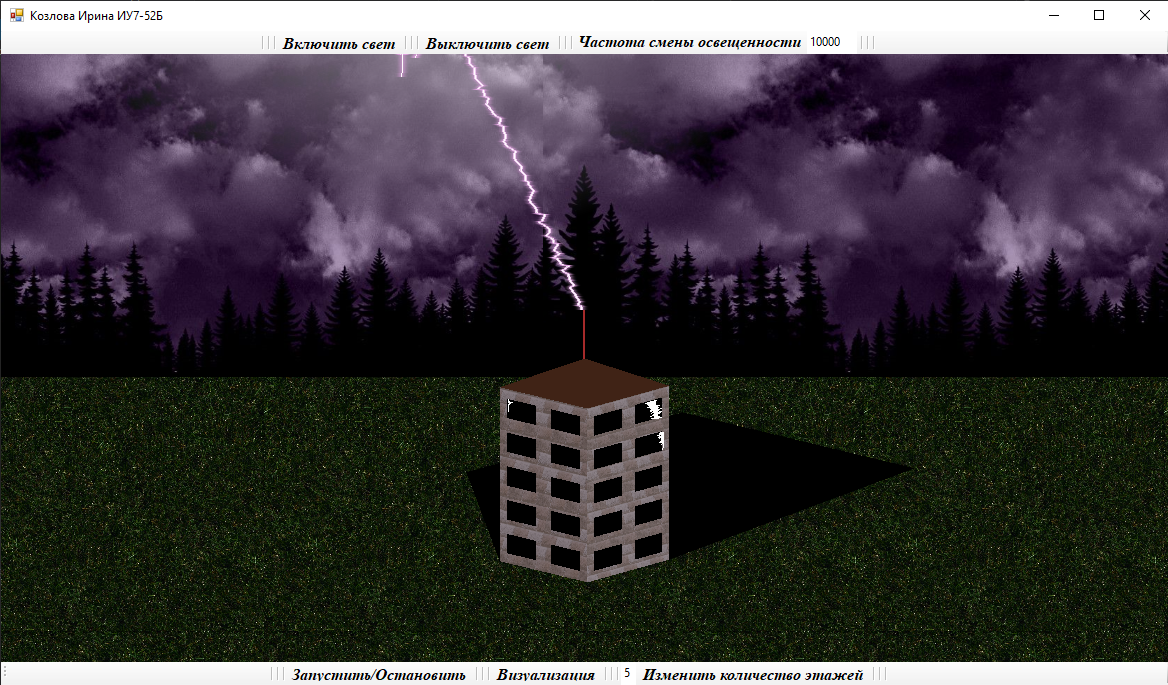
\includegraphics[scale=0.40]{img/prog_res/s1.png}
	\end{center}
	\captionsetup{justification=centering}
	\caption{Сцена 1}
	\label{img:s1}
\end{figure}

Чтобы посчитать количество лучей, с помощью которых строится сцена, необходимо посчитать количество лучей, которые испускаются из окон (равно количеству пикселей), и сложить с количеством лучей, которые пускаются во все сегменты молнии.

Количество лучей, испускаемых из всех окон, в которых выключен свет и которые ''видны'' пользователю \ref{eq:s1}.
\begin{equation}
	\label{eq:s1}
	N * S =  12 * 800 = 9600,
\end{equation}
где $N$ -- количество окон, в которых не горит свет и которые видны пользователю, $S$ -- размер окна (pазмер каждого окна -- $40 * 20 = 800$).

Количество лучей, которые пускаются во все сегменты молнии равно соответственно количеству сегментов молнии, то есть около 100 сегментов на каждую ветвь. В данном примере это количество будет равно \ref{eq:s11}
\begin{equation}
	\label{eq:s11}
	Seg * V = 100 * 1 = 100,
\end{equation}
где $Seg$ -- количество сегментов для каждой ветви молнии, $V$ -- количество ветвей.

Суммируя найденные результаты, получается, что для того, чтобы нарисовать данную сцену потребовалось $9600 + 100 = 9 700$ лучей.

Далее следует посчитать количество лучей, если бы был алгоритм обратной трассировки лучей без улучшений. 
В стандартной алгоритме требуется пустить лучи в каждый пиксель сцены. Размер сцены данной программы -- $1139 * 632 = 719 848$. 

Таким образом, можно сказать, что улучшенный алгоритм обратной трассировки лучей работает в $\frac{719 848}{9700} \approx 74$. 

Далее будут расписаны результаты по аналогичной схеме.

\subsubsection{Сцена 2}
\textbf{Описание}: Количество этажей -- максимальное, молния-лидер с большим количеством ветвей бьет в землю, во всех окнах не горит свет.

Результат представлен на рисунке \ref{img:s2}.
\begin{figure}[H]
	\begin{center}
		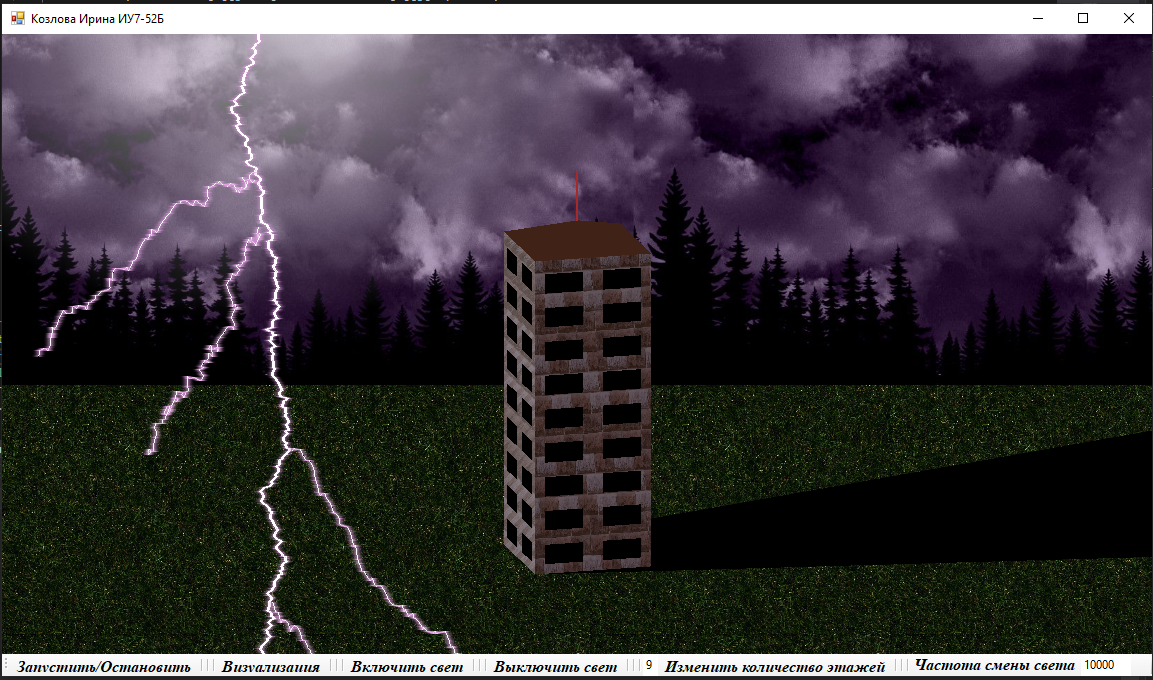
\includegraphics[scale=0.40]{img/prog_res/s2.png}
	\end{center}
	\captionsetup{justification=centering}
	\caption{Сцена 2}
	\label{img:s2}
\end{figure}

Общее количество лучей -- $ N * S + Seg * V = 36 * 800 + 100 * 5 = 29 300$.

Количество лучей при стандартном алгоритме трассировке лучей -- $1139 * 632 = 719 848$. 

Таким образом, улучшенный алгоритм трассировки лучей работает в $\frac{719 848}{29 300} \approx 25$. 


\subsubsection{Сцена 3}
\textbf{Описание}: Количество этажей -- минимальное, молния без ветвей бьет в громоотвод, во всех окнах горит свет. 

Результат представлен на рисунке \ref{img:s1}.
\begin{figure}[H]
	\begin{center}
		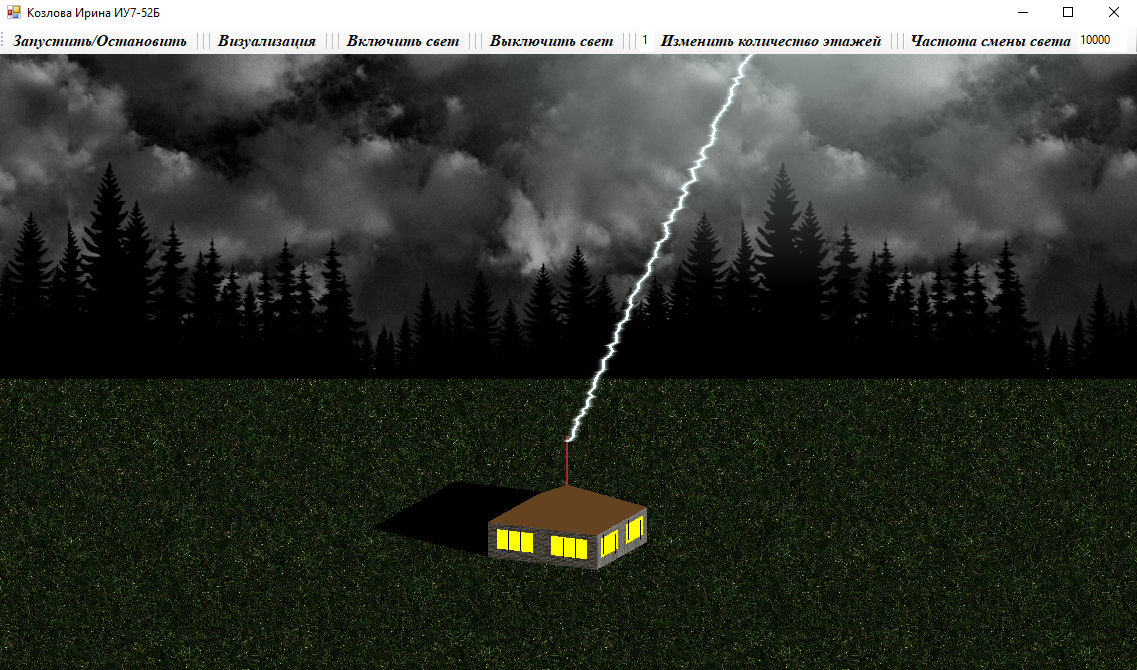
\includegraphics[scale=0.40]{img/prog_res/s3.png}
	\end{center}
	\captionsetup{justification=centering}
	\caption{Сцена 3}
	\label{img:s3}
\end{figure}

Общее количество лучей -- $ N * S + Seg * V = 0 * 800 + 100 * 1 = 100$.

Количество лучей при стандартном алгоритме трассировке лучей -- $1139 * 632 = 719 848$. 

Таким образом, улучшенный алгоритм трассировки лучей работает в $\frac{719 848}{500} \approx 7198$. 

\subsubsection{Сцена 4}
\textbf{Описание}: Количество этажей -- 5, молния-лидер бьет в землю, количество окон, в которых горит свет -- не имеет значение.

Результат представлен на рисунке \ref{img:s4}.
\begin{figure}[H]
	\begin{center}
		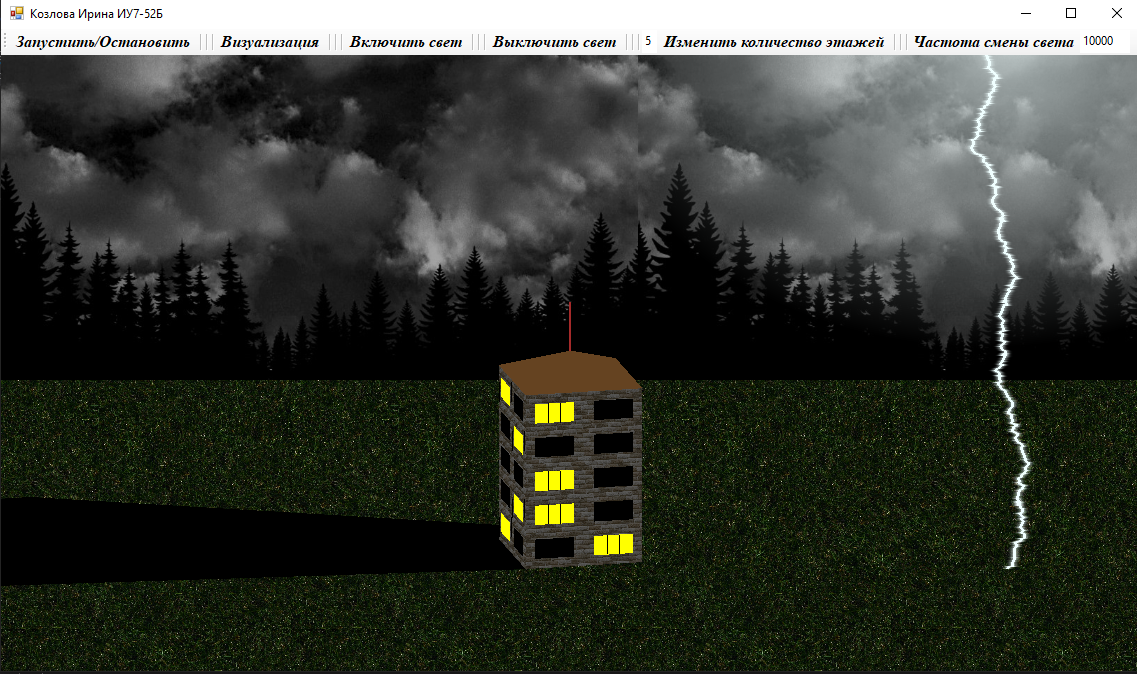
\includegraphics[scale=0.40]{img/prog_res/s4.png}
	\end{center}
	\captionsetup{justification=centering}
	\caption{Сцена 4}
	\label{img:s4}
\end{figure}

Общее количество лучей -- $ N * S + Seg * V = 6 * 800 + 100 * 1 = 4 900$.

Количество лучей при стандартном алгоритме трассировке лучей -- $1139 * 632 = 719 848$. 

Таким образом, улучшенный алгоритм трассировки лучей работает в $\frac{719 848}{4 900} \approx 146$. 

\subsubsection{Сцена 5}
\textbf{Описание}: Количество этажей -- максимальное, молния-лидер бьет в землю, во всех окнах горит свет.

Результат представлен на рисунке \ref{img:s5}.
\begin{figure}[H]
	\begin{center}
		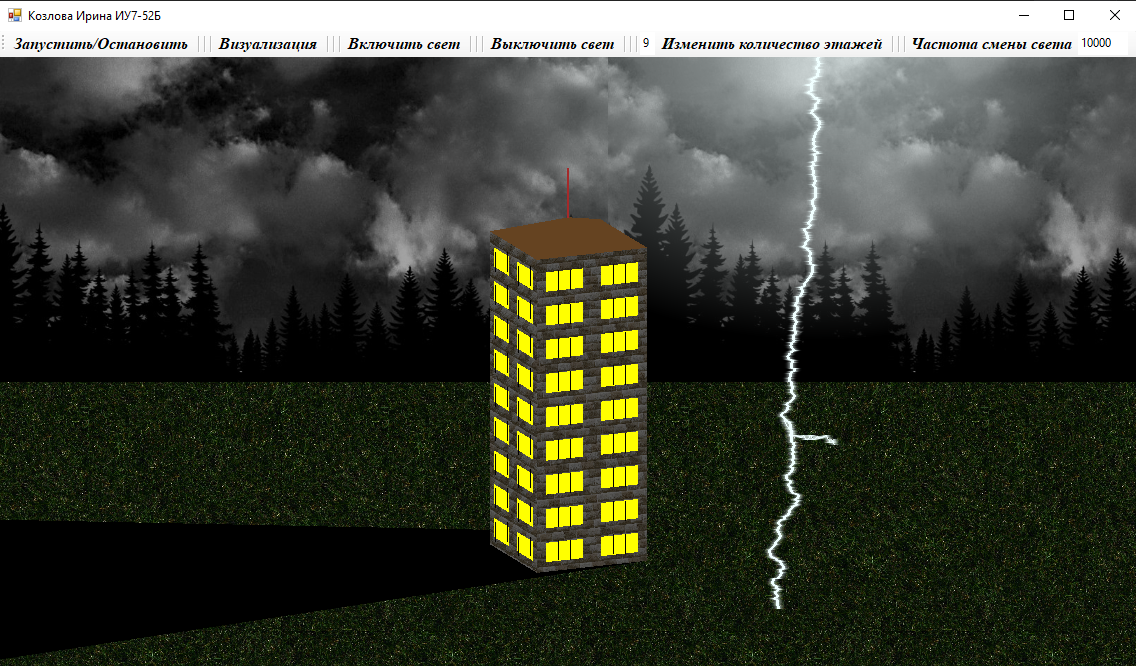
\includegraphics[scale=0.40]{img/prog_res/s5.png}
	\end{center}
	\captionsetup{justification=centering}
	\caption{Сцена 5}
	\label{img:s5}
\end{figure}

Общее количество лучей -- $ N * S + Seg * V = 0 * 800 + 100 * 2 = 200$.

Количество лучей при стандартном алгоритме трассировке лучей -- $1139 * 632 = 719 848$. 

Таким образом, улучшенный алгоритм трассировки лучей работает в $\frac{719 848}{200} \approx 3600$. 

\subsection{Замеры времени}

Замеры количества испускаемых лучей от количества окон, в которых не горит свет (учитываются только те окна, которые ''видны'' пользователю), проводились с помощью программного подсчета (переменной-счетчиком).

Результаты данных замеров приведены на графике, изображенном на рисунке \ref{img:e1}.
\begin{figure}[H]
	\begin{center}
		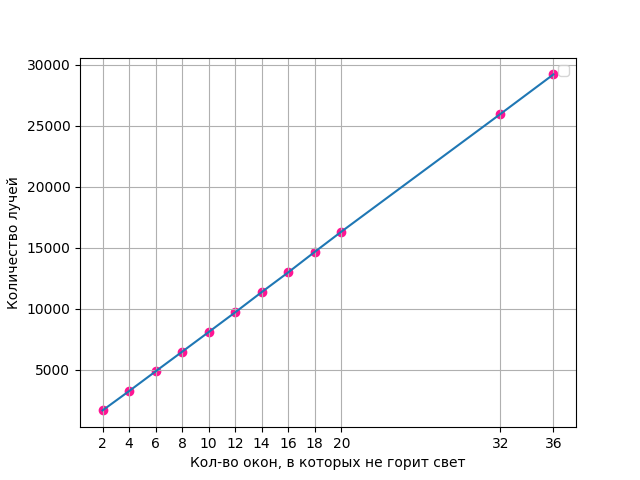
\includegraphics[scale=0.65]{img/res/e1.png}
	\end{center}
	\captionsetup{justification=centering}
	\caption{Количество лучей (количество окон, в которых не горит свет)}
	\label{img:e1}
\end{figure} 

Замеры времени построения от количества окон, в которых не горит свет (учитываются только те окна, которые ''видны'' пользователю), производились с помощью структуры DateTime \cite{csharplang1} и свойства DateTime.Now.Ticks \cite{csharplang2}.

Результаты данных замеров приведены на графике, изображенном на рисунке \ref{img:e2}.
\begin{figure}[H]
	\begin{center}
		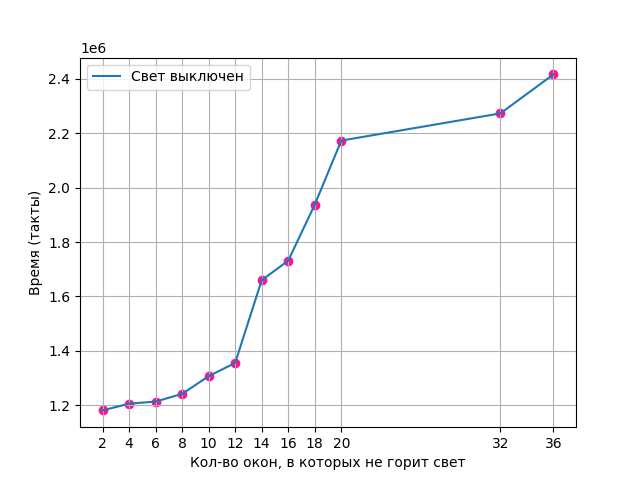
\includegraphics[scale=0.65]{img/res/e2.png}
	\end{center}
	\captionsetup{justification=centering}
	\caption{Время (количество окон, в которых не горит свет)}
	\label{img:e2}
\end{figure} 


\textbf{Сравнение времени построения сцены с выключенным и с включенным светом в окнах}

В качестве результата приведена зависимость времени построения сцены от количества этажей (количество окон, в которых выключен свет, пропорционально количеству этажей, а количество окон, в которых горит свет всегда равно максимальному количеству, то есть этажность * 8 (количество окон на каждом этаже)).

Результаты приведены на графике, изображенном на рисунке \ref{img:e3}.
\begin{figure}[H]
	\begin{center}
		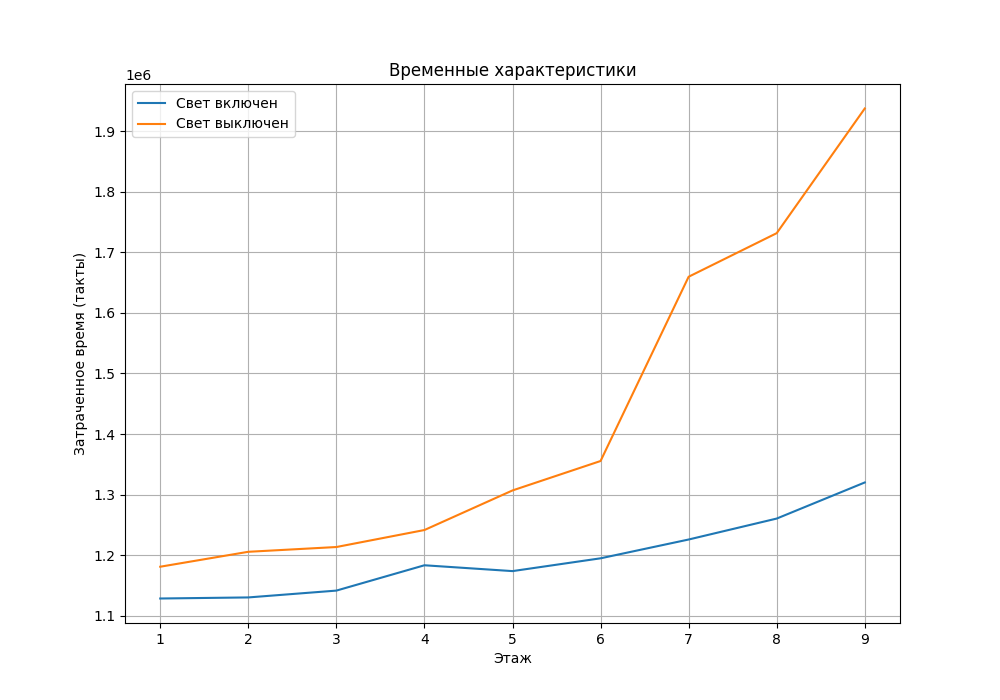
\includegraphics[scale=0.50]{img/res/e3.png}
	\end{center}
	\captionsetup{justification=centering}
	\caption{Время (количество этажей)}
	\label{img:e3}
\end{figure} 


\section{Вывод}
В данном разделе были рассмотрены примеры работы программного обеспечения, а также были вычислены и сравнены эффективности стандартного алгоритма обратной трассировки лучей и улучшенного на примере различных сцен.
 